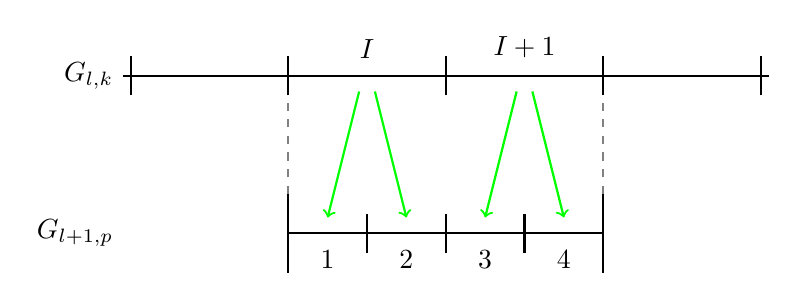
\begin{tikzpicture}
        
    % lignes horizontales
    \draw[thick] (-0.1, 2) -- (8.1, 2);
    \draw[thick] (2, 0) -- (6, 0);

    % lignes verticales
    \draw[thick] (0, 1.75) -- (0, 2.25);
    \draw[thick] (8, 1.75) -- (8, 2.25);
    \draw[thick] (2, -0.5) -- (2, 0.5);
    \draw[thick] (6, -0.5) -- (6, 0.5);
    \draw[thick] (2, 1.75) -- (2, 2.25);
    \draw[thick] (4, 1.75) -- (4, 2.25);
    \draw[thick] (6, 1.75) -- (6, 2.25);
    \draw[thick] (3, -0.25) -- (3, 0.25);
    \draw[thick] (4, -0.25) -- (4, 0.25);
    \draw[thick] (5, -0.25) -- (5, 0.25);

    % liaisons entre les maillages 
    \draw[dashed, thick, gray] (2, 0.5) -- (2, 1.75);
    \draw[dashed, thick, gray] (6, 0.5) -- (6, 1.75);

    % prolongqtion du maillage fille 
    \draw[->, thick, green] (2.9, 1.8) -- (2.5, 0.2);
    \draw[->, thick, green] (3.1, 1.8) -- (3.5, 0.2);
    \draw[->, thick, green] (4.9, 1.8) -- (4.5, 0.2);
    \draw[->, thick, green] (5.1, 1.8) -- (5.5, 0.2);

    % Annotations
    \node[left] at (-0.1, 2) {\(G_{l, k}\)};
    \node[left] at (-0.1, 0) {\(G_{l+1, p}\)};

    \node[above] at (3, 2.1) {\(I\)};
    \node[above] at (5, 2.1) {\(I+1\)};

    \node[below] at (2.5, -0.1) {\(1\)};
    \node[below] at (3.5, -0.1) {\(2\)};
    \node[below] at (4.5, -0.1) {\(3\)};
    \node[below] at (5.5, -0.1) {\(4\)};

\end{tikzpicture}